\documentclass[sigtbd]{sigtbd17-style}

\usepackage{amsfonts}
\usepackage{censor}
\usepackage{color}
\usepackage{graphicx}
\usepackage{hyperref}
\usepackage{xspace}

% \todo macro
\newcommand{\todo}[1]
{{\bf\color{red}[#1]}}

\newcommand{\premium}{Gold Plus\xspace}

\begin{document}

\title{\todo{Something} presents OpenAdcess}
\maketitle

\begin{abstract}
  In this paper we examine an alternate funding model for open access papers.
  Through modest modifications to the ACM Digital Library and the addition of
  paper sponsorships we can make the entire corpus of ACM works free to the
  public.
  We also peer into a chilling future that only we can prevent.
  Will we stop the ACM from encroaching on our everyday freedoms?
  Continue existing and participating in reality to find out!
\end{abstract}

\section{Introduction}
Open access is a movement to make papers and other research contributions
freely accessible to the general public \cite{oa}.
The ACM has been working for some time to achieve the open access dream but
have found this dream to be prohibitively expensive.
As such, we have required authors to opt-in to open access by paying the cost
themselves \cite{auth}.
However, we have found a way to provide open access papers at no cost to the
authors by adopting the techniques employed by various websites and
publications that manage to distribute content for free.

Section~\ref{sec:related} details techniques used by other services to achieve
free downloads and paper distribution.
Section~\ref{sec:lib} describes the upcoming changes to the Digital Library to
bring it up to the current standards for download portals.
Section~\ref{sec:sponsors} adapts techniques from tabloids to ensure that
the papers themselves are profitable.
Section~\ref{sec:future} provides work from a future that directly results from
a present that includes the present work.



\section{Related Work}
\label{sec:related}

Download.com \cite{download-com} provides free downloads of popular programs to
the public.
We borrow their idea of using misleading advertisements to trick users into
downloading programs they may not want in \autoref{sec:fake}.

Rapidshare \cite{rapidshare} was a website that provided rate limited free
downloads while simultaneously selling a paid download service that was
superior to the free tier.
This technique was meant to entice users to pay for the service.
Unfortunately, as Rapidshare no longer exists it seems that this technique
alone is insufficient to cover the costs of running a download service.
However, we still employ the technique as explained in \autoref{sec:limit} as a
supplemental revenue stream.

\todo{Harvest paper} and many other free rags employ heavy use of in paper ads,
native ads, and classifieds.
We also adopt these techniques to embed in all of our papers in
\autoref{sec:sponsors}.

Edsger W. Dijkstra has previously proposed the revolutionary idea of
capitalizing mathematics \cite{cap-math}.
We expand on this idea with our branded mathematical objects in
\autoref{sec:brands}.


\section{Digital Library}
\label{sec:lib}
Shady websites have long managed to monetize free content downloads.
Below we detail the ways in which we can follow their example to provide free
access to papers and liberate the ACM reader from covetousness.

\subsection{Fake Download Buttons}
\label{sec:fake}

Fake download buttons are a staple of modern download websites. They really
class up the web. Reifying, elegizing, and idealizing nature, these abstract
forms  direct the downloader's attention away from the url
to the ad-serving service to which the button points. A deceptive
d\'{e}tournement, the placement of these blissed-out buttons
challenges browsers to consider whether they really want to download the paper.
They could, after all, choose to abandon their line of inquiry and instead
watch their field's evolution vicariously through mainstream media, which cuts
down on the ACM's hosting costs.

By allowing advertisers to buy space on our digital library with which to
create ads that look like download buttons, advertisers can deceive users into
clicking an ad.
The advertiser and the ACM both profit off of these deceptive ads as the user
is redirected to see the advertiser's product while the ACM gets the revenue
for an impression. Some regulators have questioned this practice. But we
believe it is a win-win-win for consumers \footnote{Gary Cohn, the director of
  the National Economic Council, stressed in an interview with \textit{The Wall
Street Journal} compared a website without fake-download buttons to the menu at
P.J. Bland's: ``This is like putting only health food on the menu, because
unhealthy food tastes good. But you still shouldn't eat it because you might
die younger." The menus of a free society, in his reckoning, should include
both unhealthy and healthy items, and they should be labeled and priced
identically. It should be impossible for consumers to access independent,
third-party statistics about menu items. ``We believe our customers are
informed and engaged, and we trust that they are smart enough to make the
decisions that are right for them. We don't want the government treating them
like dotards," Gary Cohn said while spraying an unlabeled can of spray cheese
into his mouth.}.


Additionally, these download buttons could be functional in that they download
\textit{something}, but the ACM digital library will not impose any
restrictions on what may be downloaded from these fake buttons.
Therefore, advertisers are welcome to serve us infected PDFs or straight up
executables.
It is our position that users must be intelligent enough to hunt down the
proper download button, and that academics can learn valuable security
practices when they know that others could steal their research through
malicious downloads on the digital library.

To subvert ad blockers, the ad content will be natively hosted on the ACM
digital library as well.
Therefore, ad blockers will be unable to determine which requests are ad-related.

Additionally, we are revolutionizing the fake download practice by dynamically
randomizing the position of the actual download button.
Like serving ad content natively, this will make ad blockers functionally
useless as there will be no way to differentiate between ad content and ACM
content, providing users with instruction on the contingency of fate.
Moreover, this randomization makes it much harder for the user to learn the
positioning of the ads and therefore we hope to drive more clicks to our ad
partners and generate more revenue for the ACM.

Lastly, we are working on a proposal that will greatly reduce ACM hosting
costs, namely we  will replace the only real download button with a fake one.

\subsection{Rate-Limited Free Downloads}
\label{sec:limit}
Free download sites figured out long ago that you can make people pay for an
otherwise free product by making the process of obtaining that free product
difficult.
Therefore, we will split our digital library downloads into two tiers, the free
tier and the \premium tier.

The free tier will only allow downloads at slow speeds and no more than one
paper per day.
Additionally, the user will be required to stare at a screen compelling them to
upgrade while a counter decrements for 10 minutes before the download button is
clickable.
If the engagement of the user---monitored via gaze tracker and wearable
heart-rate monitor---falls below the Zone of Synergy\texttrademark, the counter will be restarted.
The \premium tier will allow unlimited downloads along with an upgraded
experience: the countdown clock will have ads replaced by a sponsored message
thanking you for upgrading and will feature a \premium digital clock face.

\subsection{Outsourced Captchas}
When a user requests a paper download, they will be required to submit a
captcha.
While many websites use captcha to prevent automated abuse, we see an
opportunity to profit.
We provide an API to botnets with which they may submit captchas to be
displayed to users attempting to download files.
Their responses to these captchas are sent back to the botnet thus allowing the
botnet to proceed with whatever attack the captcha was preventing.
We believe we can sell this human captcha solving service for a few cents per
captcha.

Users will not question the presence of captchas on the digital
library as they have already been conditioned to fill captchas for all sorts of
free services.
As such, we do not believe that our user base will know that the ACM is
slinging captcha solutions on the side.

\subsection{ACM Digital Library Toolbar}
Every ACM paper will be distributed as an executable.
Running this executable will ``install" the paper to the user's desktop.
The only purpose of the install is to push the ACM Digital Library toolbar on
the user.
While the toolbar itself is optional, its installation is opt-out.
The ACM Digital Library toolbar will be installed for the user's web browsers where it
will follow them from site to site collecting information about their browsing
habits.
We will provide this information to our partners for a nominal fee who may use
this user data to curate a product-based lifestyle that will make our readers' lives
more relevant to advertisers.

Additionally, the toolbar will constantly mine bitcoins on the user's machine
and send the mined coins to the ACM's wallet.
If the user has a GPU, the development drivers will be silently installed along
with the toolbar to enable GPU mining.
We hope that one day the ACM mining pool becomes so large that we become a
dominant player in the Bitcoin economy.
If we ever reach a simple majority of the mining power, we WILL mount a 51\%
attack to seize control of the network for our own financial gain.

In order to comply with New Jersey's backwards laws about involuntary Bitcoin
mining \cite{tidbit}, all New Jersey residents will be preemptively banned from
the ACM Digital Library and the greater academic community.

\subsection{Impact Factometer}

Researchers want their projects to have meaning and impact. Administrators like to market their department's product as meaningful and impactful. But how can researchers tell their work is saving the world?

Simple. Once a quarter, the Ricketts family convokes Gary Cohn, Dennis Rodman,
Colonel Sanders, and the rest of the Economic Advisory Council at Chicago's
historic Wrigley Field to make use of the stadium's native Noiseometer. As Pat
Hughes reads the papers over the PA , the council---taking especial care to
note the presence of key phrases like ``cross-promotional deal mechanics
revenue streams jargon synergy" and ``a strategic planning initiative\ldots
with a focus on strategic dynamism"---emits cheers in proportion to its
perception of the paper's impact, and these cheers are registered on the
Noiseometer, which assigns metrics of impact to each paper, as shown in Figure~\ref{fig:noiseometer}


\begin{figure}
  \centering
  %https://archive.org/details/414803main_0203243
  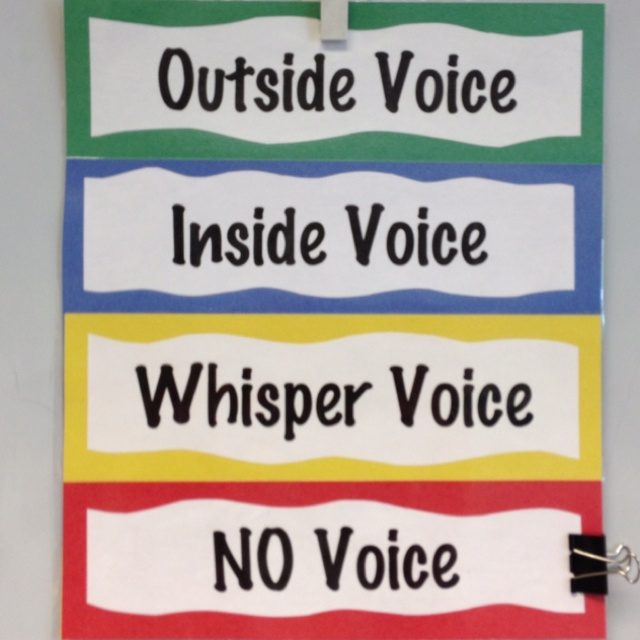
\includegraphics[width=0.45\textwidth]{figures/noiseometer.jpeg}
  \caption{A model-year 1985 Noiseometer, prized by collectors for its muted
  design that limns adumbrations of sound. The paper in which these meetings
were proposed was met at the first such convening of the Council with a cheer
so loud it registered a ``Nowhere Permissible Voice" \todo{maybe think of
something better} (not shown) on this scale.}
  \label{fig:noiseometer}
\end{figure}


These metrics empower our research partners to be certain their research is having a real-world impact.  It is important for researchers to know that they don't risk deactivation or exile if they remain on track.


\section{Paper Sponsorships}
\label{sec:sponsors}
In addition to ads on our Digital Library, we will also be adding
advertisements to the papers themselves.
These advertisements will come in many forms, including standard banner
advertisements as well as increasingly popular native advertisements.

\subsection{Call for Advertisements}
Reach the largest holistic-minded audience in the entire northeastern United
States with an ad in the next ACM edition.\footnote{Wisdom disputes this claim, but we have the narrow computational tools to prove our publication and community have way more holism.}
Our readership is mostly devoid of energy vampires and is therefore suitable
for empath advertisers.
Where IEEE uses Western proof verification techniques, our broad minded
audience validates mathematical claims in an intuitive holistic manner and will
bring that same spirit into evaluating the claims of your advertisements.
Our readers will engage with your brand through meditation and other
surprises.

\subsection{Banner ads}
Web surfers today have become accustom to seeing banner ads on their favorite
websites.
Therefore, we will be incorporating these advertisements into all of our
papers.
Advertisements can be easily inserted into existing \LaTeX\ papers through the
use of the \texttt{\textbackslash figure} and \texttt{\textbackslash figure*}
constructs.
Of course, advertisements using the two column \texttt{\textbackslash figure*}
construct will be considerably more expensive than their one column brethren.
A standard single column ad can be seen in \autoref{fig:law} while a
double-wide can be found in \autoref{fig:usa}.

\begin{figure}
\centering
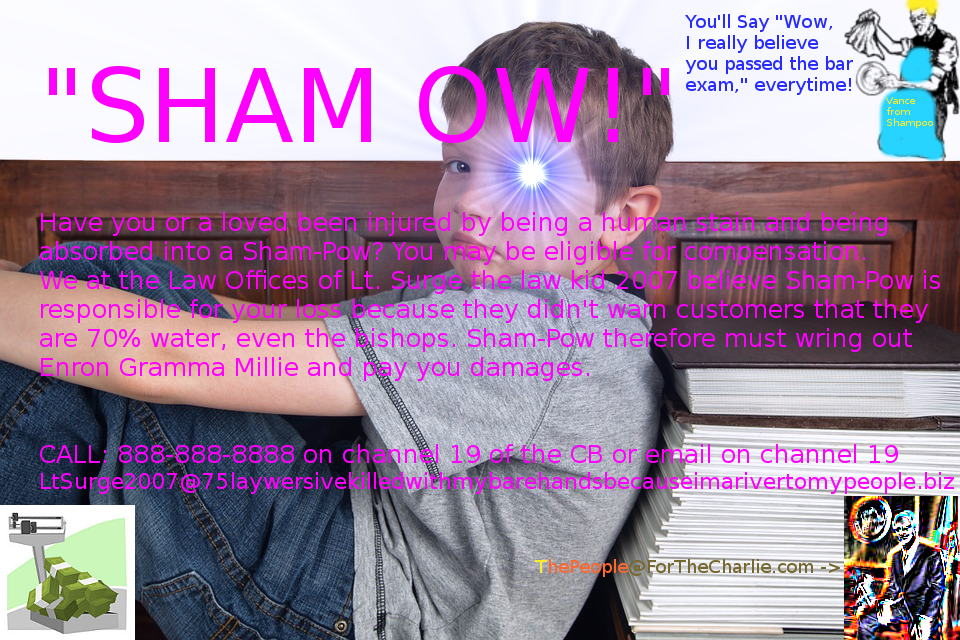
\includegraphics[width=0.45\textwidth]{figures/law-kid-ad.png}
\caption{Get your settlement today \cite{med-scale}!}
\label{fig:law}
\end{figure}

\begin{figure*}
\centering
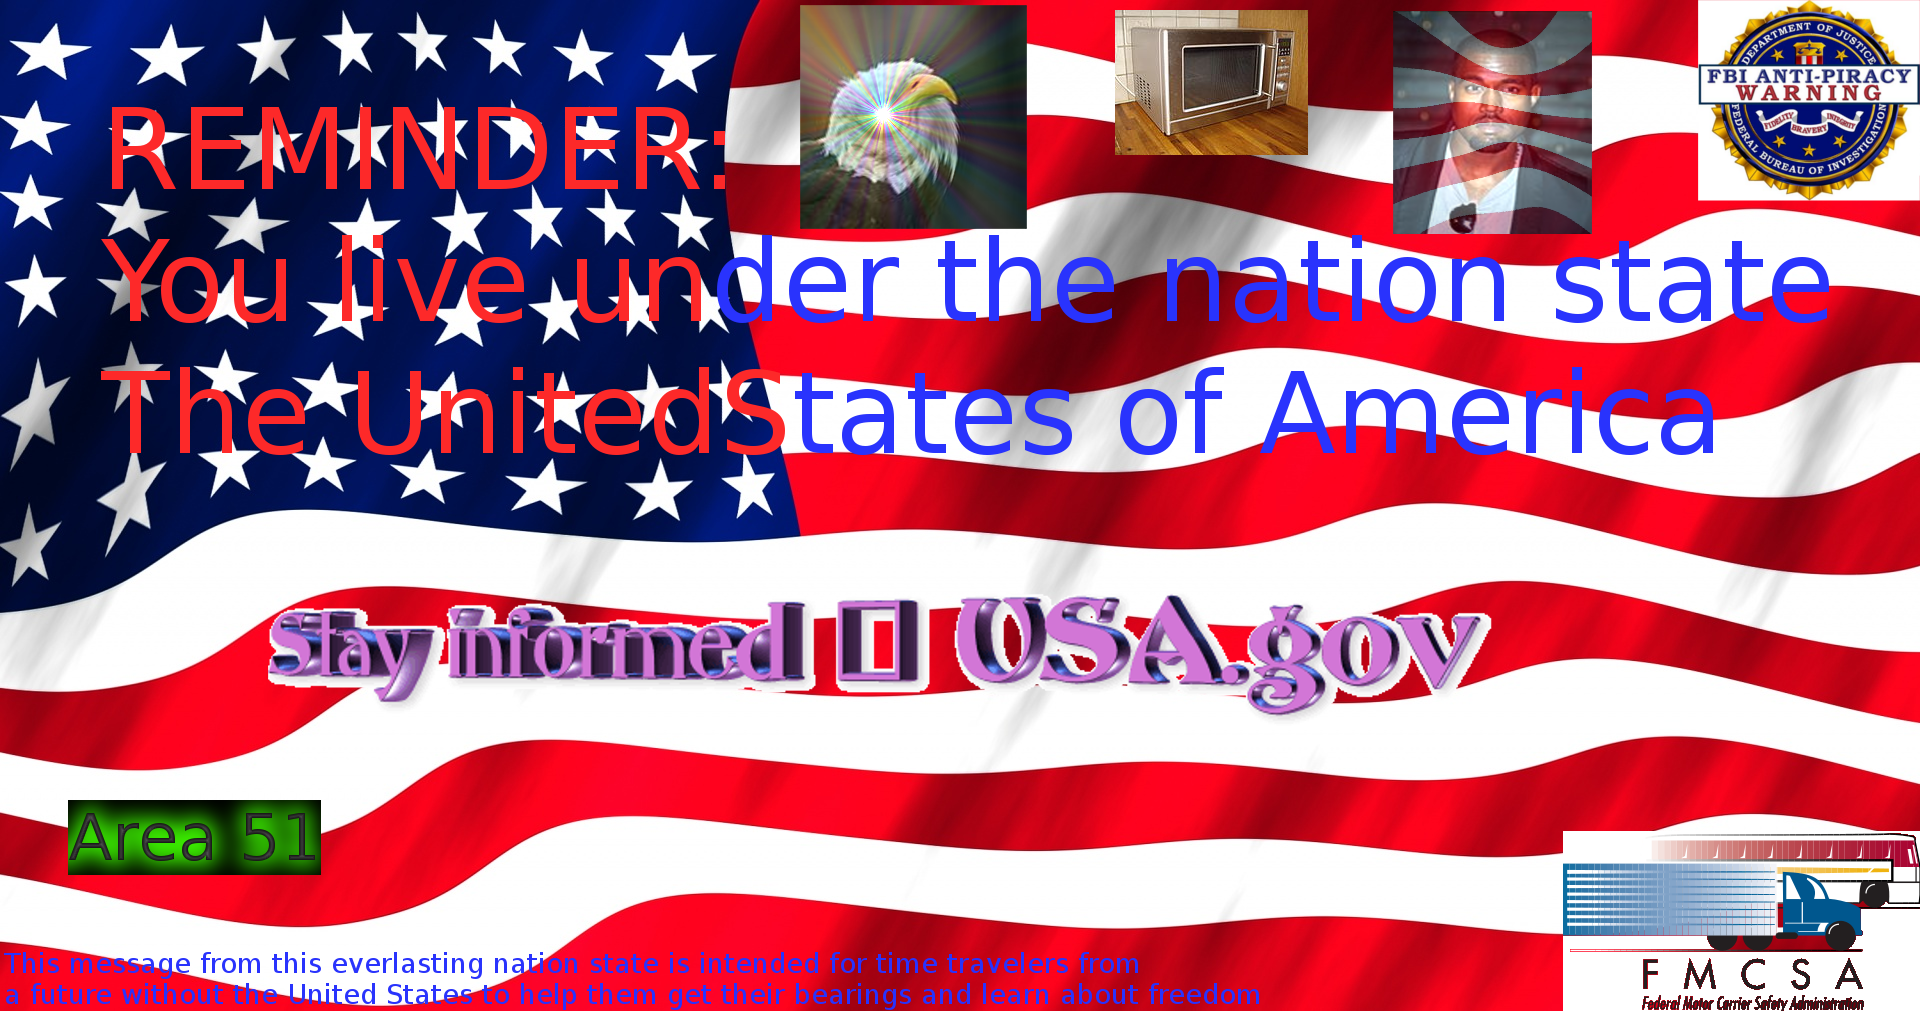
\includegraphics[width=0.95\textwidth]{figures/usa-ad.png}
\caption{We have near absolute power over you \cite{eagle, kanye, microwave}!}
\label{fig:usa}
\end{figure*}

For an additional fee we will also allow advertisers to embed autoplaying audio
into their paper ads.
While we aren't currently sure whether or not the PDF specification allows
this, we believe that there are sufficiently many ACM loving PhDs at Adobe to
get this change  pushed into the spec.

\subsection{Ad Enhanced Fonts}
Computer Modern is a staple of today's papers, but we believe that this font can
be monetized.
By replacing the characters in the default \LaTeX\ font with corporate logos
we can convey the same information in an ad enhanced way. The inspiring example of Claude Shannon proves it!



During each call for papers we will also put out a simultaneous call for
logos where companies can bid on desirable letters.
To avoid a Wingdings situation \cite{wingdings}, we require that the company
logo is a stylized version of the letter being replaced.


\subsection{Native Ads}
Native advertisements are advertisements meant to be disguised among the normal
content of a publication.
They are written in the same style as the publication and appear alongside
unsponsored content in an attempt to make the reader believe that they are
reading the original publication and not an advertisement \cite{native}.

At paper registration time, authors will be given ad copy to integrate into
their work.
Each paper is required to have at least one section advertising the product
that was assigned to the research project.
As these ads must be indistinguishable from the rest of the paper, an
advertisement that is recognizable as an ad will result in the rejection of the
paper.
The ad section must be at least one page long, but there is no upper bound on
native ad length.
We recognize that this will eat into the page limits of some conferences so we
will allow authors to deduct the length of the native ad from their total paper
length provided that the length of the native section alone exceeds the total
page limit.
Authors can claim this deduction by filing a Form 8843 with their paper
submission.

\subsection{Branded mathematical objects}
\label{sec:brands}
We believe there has been a missed opportunity in the field of mathematics to
increase brand awareness.
Therefore, we propose branding mathematical objects by associating every single
set with an individual brand.
Brands can purchase large collections of sets at a discount.
While most sets are cheap, some more famous sets will be priced higher to
reflect their higher market value, similar to domain names.

Authors referencing any given set must reference the brand of the set any time
the set is referenced, regardless of the format the set is presented  in.
Additionally, royalties must be paid to the owner of the set.

We are excited to announce that our first partner in this endeavor will be
Chili's Grill \& Bar,\footnote{Pronounced: \texts{Kill me's} The chill of severity and emptiness.} who has purchased the rights to the set of natural
numbers.
From here on, authors must refer to this set as the Chill's Grill \& Bar Set of
Natural Numbers \(\mathbb{N}\).

\subsection{Investor Science Dispute Settlement}
We have founded an Investor Science Dispute Settlement (ISDS) court to protect
businesses from results that may damage their reputation or profits.
If a research project is found to be damaging, the authors must either retract
the paper or pay a settlement equal to the estimated losses suffered by the
company.
For example, if some agitator finds that the complexity class PLS is in PPP
relative to some oracle, they will dash the hopes of the typical Sparrow Soap
consumer, leading to hygiene neglect.
Therefore, Sparrow Soap may use the IADS court to mitigate their losses from
this finding.
Moreover, since Sparrow Soap owns both of these complexity classes as defined
in section \autoref{sec:brands} their assets will lose value and
this loss must be compensated by the offending authors.

Several ``bloggers" and fuddy-duddies fixated on a staid notion of ``truth" (lacking the agility and dynamism that characterize a proactive, change-driven science) have deigned to argue that this arrangement gives particular corporations undue influence over science and could lead to corruption. These agitators are, of course, anti-science zealots who fail to realize the emancipatory potential of this settlement system. Much as the visionary rulings of Anthony Kennedy and others have opened up our politics to make it more responsive to democratic speech, ISDS will make science more responsive to the needs of democratic actors, like 501(c)(4) ``social welfare" nonprofits. Welfare! It will democratize our understanding of reality, taking science out of the smooth, mildly scented ivory tower and cramming it into the ad-plastered public square. Science is agoraphobic but its future is in the agora of the brainscape---the marketplace of ideas---so (to coin a term) ISDS is the deagoraphobification of science. Science cannot ignore society. Science must come to where the flavor is.

What of the science that does get published? The agents who do get economically controversial results published---the humble, modest, yeoman-scientist free agents---are likely to be powerful entities in a society with concentrated private economic power, some argue. How is that democratic? Well, Madison got it right. It's not only democratic, it's the purest form of democracy: the ``mischief of the factions." Simply put, ISDS provides a powerful mechanism of checks and balances. If Hot Packets wants to get their signature snack food placed on the government's food pyramid, it would need peer-reviewed science attesting to its beneficial health effects (such as an appearance on the Doctor Conflict-of-Interest show, where the titular doctor attests to its miracle superfood status, or a research paper). To appear in print, it would have to pay off claims from competing superfoods such as Berry Loops or Jazz Flakes. The system works! But, say, if the parent companies of all products for sale wish to merge, research touting the consumer benefits and questioning Robinsonian labor market monopsony would have little trouble passing ISDS. Approved ideas get approved quickly, and the system works!

ISDS also applies to scientists in their personal lives. If a scientist, for instance, posts to social media video of an alleged bad encounter with an internet service provider's customer service representative or video of hose water burning---and ISDS tribunal statisticians (employees of the ISDS corporate community, on rotation) determine that, as a result of these actions, shareholders lost value---then the economic terrorists promulgating this ticker-tanking tripe will have to compensate all shareholders for the drop in share price, as well as the social media platform monopoly's shareholders (if applicable; scientists should not be using free, distributed social networks but may use privately held proprietary platforms) for the shame they've brought to the platform even if share price was unaffected. This way, the integrity of the scientific process is protected---and scientists represent science with honor---in all spheres, not just peer-reviewed journals.   

\subsection{ACM Classifieds}
For additional funding we allow individuals to take out classified ads in the
following sections.
To keep costs low, the ACM does not vet any classified postings.

\paragraph{Dropped Packets}
Dropped Packets serves as the traditional missed connections section of the
classifieds. While this could be used to contact that cutie from the latest
While this could be used to contact that cutie from the latest conference, we
believe that it could also be used to publicly shame those who miss meetings.

Sample: Missed Connection: Lost Tofutti Cutie at last conference, fell behind the freezer before I could read it. No reward. I just want a witness to my experience.

Sample: ``Damn it Deborah, you were supposed to bring bagels to the DARPA
Tactical Anti-\censor{blank} HAVE BAGEL Infiltration \censor{long blank}
(DTA\censor{b}HBI\censor{bb}) meeting!"
Sample: I was hiding in your closet at 54 Bishop Allen Dr. # 2 and you were home and you took a shower but you grabbed wrinkled clothes from your laundry hamper and didn't access your closet, and I hadn't eaten anything but moths for many hours, so I slipped out of your home but just know you are loved.

\paragraph{Job Queue}
The Job Queue section contains odd jobs for trained Computer Scientists looking
for instant internet income.
Those who pay extra will get a free AirDancer\footnote{Placed at the discretion
of the ACM in the ACM AirDancer Oasis in the Black Rock Desert in Nevada in
solidarity with the aliens illegally detained in Area 51. The AirDancers may
be used by the aliens to communicate with their home world about the status of the part needed to keep the AirDance of the cosmos going.}!




\paragraph{Overclock}
Overclock is a section for performance enhancing drugs tailored for computer
scientists.
This section is mostly targeted at the Hacker News \cite{hn} crowd who exclaims
the benefits of small amounts of LSD for enhancing productivity at work
\cite{microdose, lsd-song}.
Although we can't promote the use of illegal drugs our editor is so strung out
on ``road cheese" that she won't notice.
% http://www.forbes.com/sites/robertglatter/2015/11/27/lsd-microdosing-the-new-job-enhancer-in-silicon-valley-and-beyond/#323d0dab114d

\subsection{Check Scams}

Digital is the new normal. Digital is the new ubiquity. Digital is the new cuddling. Digital is the new word we use to paper over our alienation with the capitalist mode of production at a time when socialism is possible.

We are now living in a world of 0s and 1s---or, if you prefer, sharks and minnows. The transformative power of this new digital world has been fully realized. Nothing can get more digital. It's either digital or it's not. And by now everything that's ever going to be digital has already become digital. We must accept this fact of this hardscrabble, accept-or-be-accepted world.

With our new digital world comes new digital innovations. Every brand, every person, and every personal brand is now a digital native. Digital is native and native, digital. Every transistor will be able to heal itself without consulting a physical medicine man. Big data, hot data, slow data, medium data, dirty data, long data, cold data, transient data, live data, cubed data, and target-rich data. But data is just a story, a narrative, and though every brand tells an authentic story, a brand is more than a story. The universe is not a story.

Thus, we will need to move beyond digital because digital is just story-telling. What matters is physical. Action potentials sparked by sensory inputs---sight, taste, ESP---and other action potentials. Statues of Jesus being carried by helicopter. Nothing is more authentic for consumers than the physical, than an action potential. In a world where everything is phony, only an action potential---even one involved in the process of telling a brand's story---is real.

Digital embodies the lifestyle and personality of the ACM author. But the ACM author exists in a physical space. Prior to the open-adcess revolution, the ACM author had to transact in this physical space to release a paper (digital locker room talk) in an ACM journal (digital locker). The revolutionary open-adcess model is America-first, digital-second. Now authors need never leave their digital hidey-holes by transferring funds to the ACM and, through fractional-reserve banking, creating physical changes in the non-digital sectors of our digital economy. 

But an author need not remain ensconced in the stately pleasure-dome of digital. In fact, when an author chooses to transact in the physical space, the open-adcess model empowers the author to not only avoid paying the publishing fee but also to get on the road to getting paid for their articles because authors deserve more. Recent accounting innovations surveyed in two review articles and one major motion picture ["Consumer Information: Fake Checks"
https://www.consumer.ftc.gov/articles/0159-fake-checks; "Counterfeit Check Scams: CONSUMER ALERT" http://www.michigan.gov/ag/0,4534,7-164-17337_20942-176356--,00.html; \textit{Bridget Jones's Check Scam} distributed by Universal Pictures] enable the ACM to write large checks to authors. In return, authors simply have to write a small check to cover transaction fees before the large check clears.

\begin{figure}
\centering

\includegraphics[width=0.45\textwidth]{figures/ad.jpg}
\caption{Have you seen this boy?}
\end{figure}


\section{Future Work}
\label{sec:future}
This future work appears in SIGTBD \todo{citation to future
paper edition}.

\todo{All crazy future ideas go here.
Verification snacks, etc.}

\subsection{Introduction}
\paragraph{Introduction} An introduction is an explanatory section of a document that introduces the topic discussed in the document and presents a thesis statement.
\paragraph{Antithesis} Think about it, man. There is not introduction. We just see bad writing, cast as we are into this broken world.
\paragraph{Sublation} The introduction, some may argue 

We think introductions leave those catching up with a field disoriented. More theater than truth, these sections do little to erase the veil of nonseeing from the student's mandatory raised unibrow, but -- please take a moment to recognize the taste of ACM Cola or the cool, refreshing ACM technology deity which (for all you just tuning in who forgot your mandatory religious training) we call Jerry -- the introduction 

the boundless territory of 


As you may recall from \todo{sublation}, the engineers have ended the industrial dictatorship of the captains of finance as a matter of convenience

\subsection{Premium Edition}
To those who dislike the ads they see, ACM will offer a premium version for
2000 Linden dollars per year \footnote{In the future Linden dollars are the
one true world currency.
The value of 2000 L\$ in today's United States Dollar is currently unknown.}.
Unfortunately, due to high credit card processing fees we must still show ads
to premium edition subscribers.
However, these ads will be for more expensive products targeted towards those
with more ``refined" tastes.
We hope to solve this issue in the future with the creation of Bank of ACM.

\subsection{Ad-Free Edition}
For those who are physically able and enthusiastic about being part of
something big, the ACM offers ad free papers in exchange for manual labor at
your local ACM work dungeon.
This labor involves turning a very large crank around a pivot point in the
floor.
The crank is attached to a magnet spinning in a metal coil to generate the
necessary electricity required to power our servers.
However, all of this electricity is used to power electric lumbar support for
OSHA employees in exchange for their continued appreciation of the safe
practises within our work dungeons.
Two months of full time service provides access to five ad-free papers.
Professors may opt to have their graduate students turn the crank in their name
to count towards their service.

Our throwback dress code seen in \autoref{fig:mill} captures the timeless
values that power ACM while making escaped grad students easy to identify.

Students who fail to be creative, stay connected, and keep inventing at the
dungeon will be required to perform additional labor in what we call ``invited
service" before their advisors can receive their ad-free papers, as seen in
\autoref{fig:horse-mill}.

Some enterprising students like the one in \autoref{fig:vr-mill} are testing
new virtual reality mills that allow the student to reshelve the digital
library while they turn the mill.

\begin{figure}
  \centering
  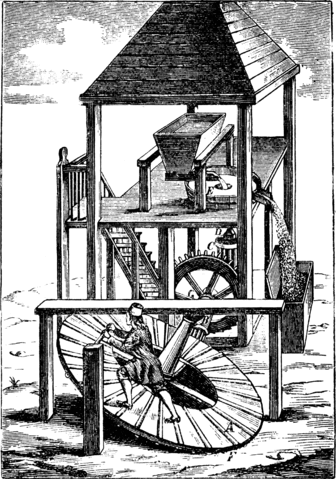
\includegraphics[width=0.45\textwidth]{figures/mill.png}
  \caption{ACM work dungeon mill powered by 5th year grad student. Notice how our graduate students show great vigor and -- auscultate away! -- don't sound consumptive.}
  \label{fig:mill}
\end{figure}

\begin{figure}
  \centering
  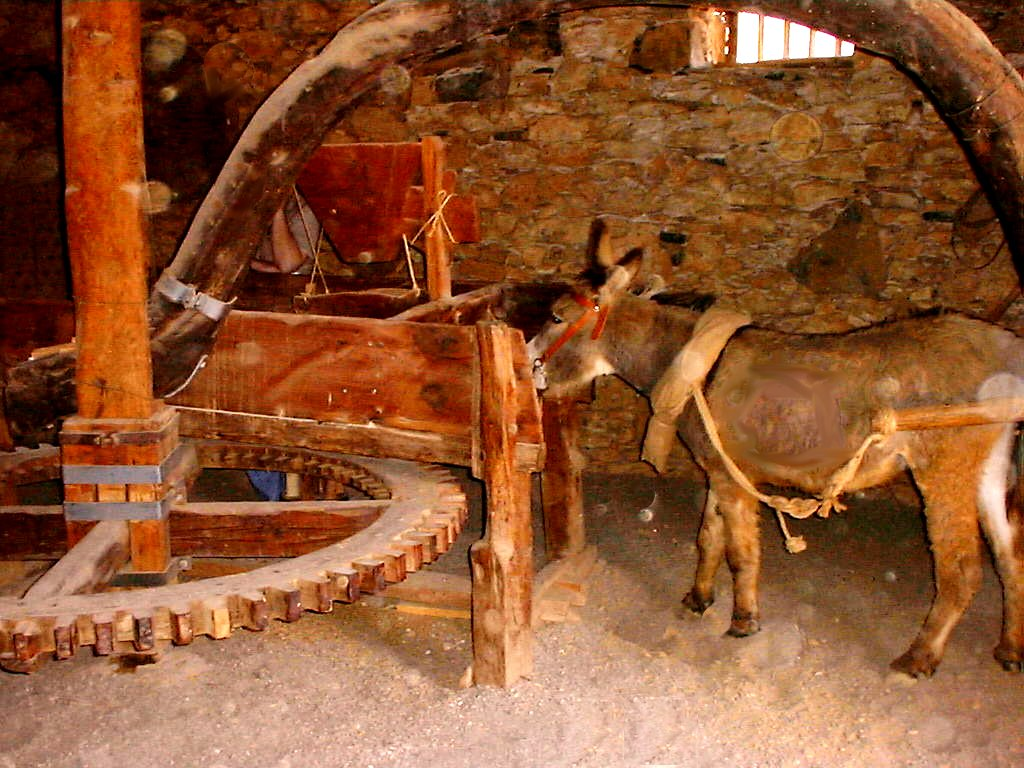
\includegraphics[width=0.45\textwidth]{figures/horse-mill.jpg}
  \caption{12th year grad student sentenced to extra
  month in work dungeon for insufficient commitment to the mission of advancing
computing as a science and profession.
Not only is he a lifetime ACM member, but he's a lifehacker!  Shown here in his
ergonomic harness and standing desk.
OSHA would be proud.}
  \label{fig:horse-mill}
\end{figure}

\begin{figure}
  \centering
  %https://archive.org/details/414803main_0203243
  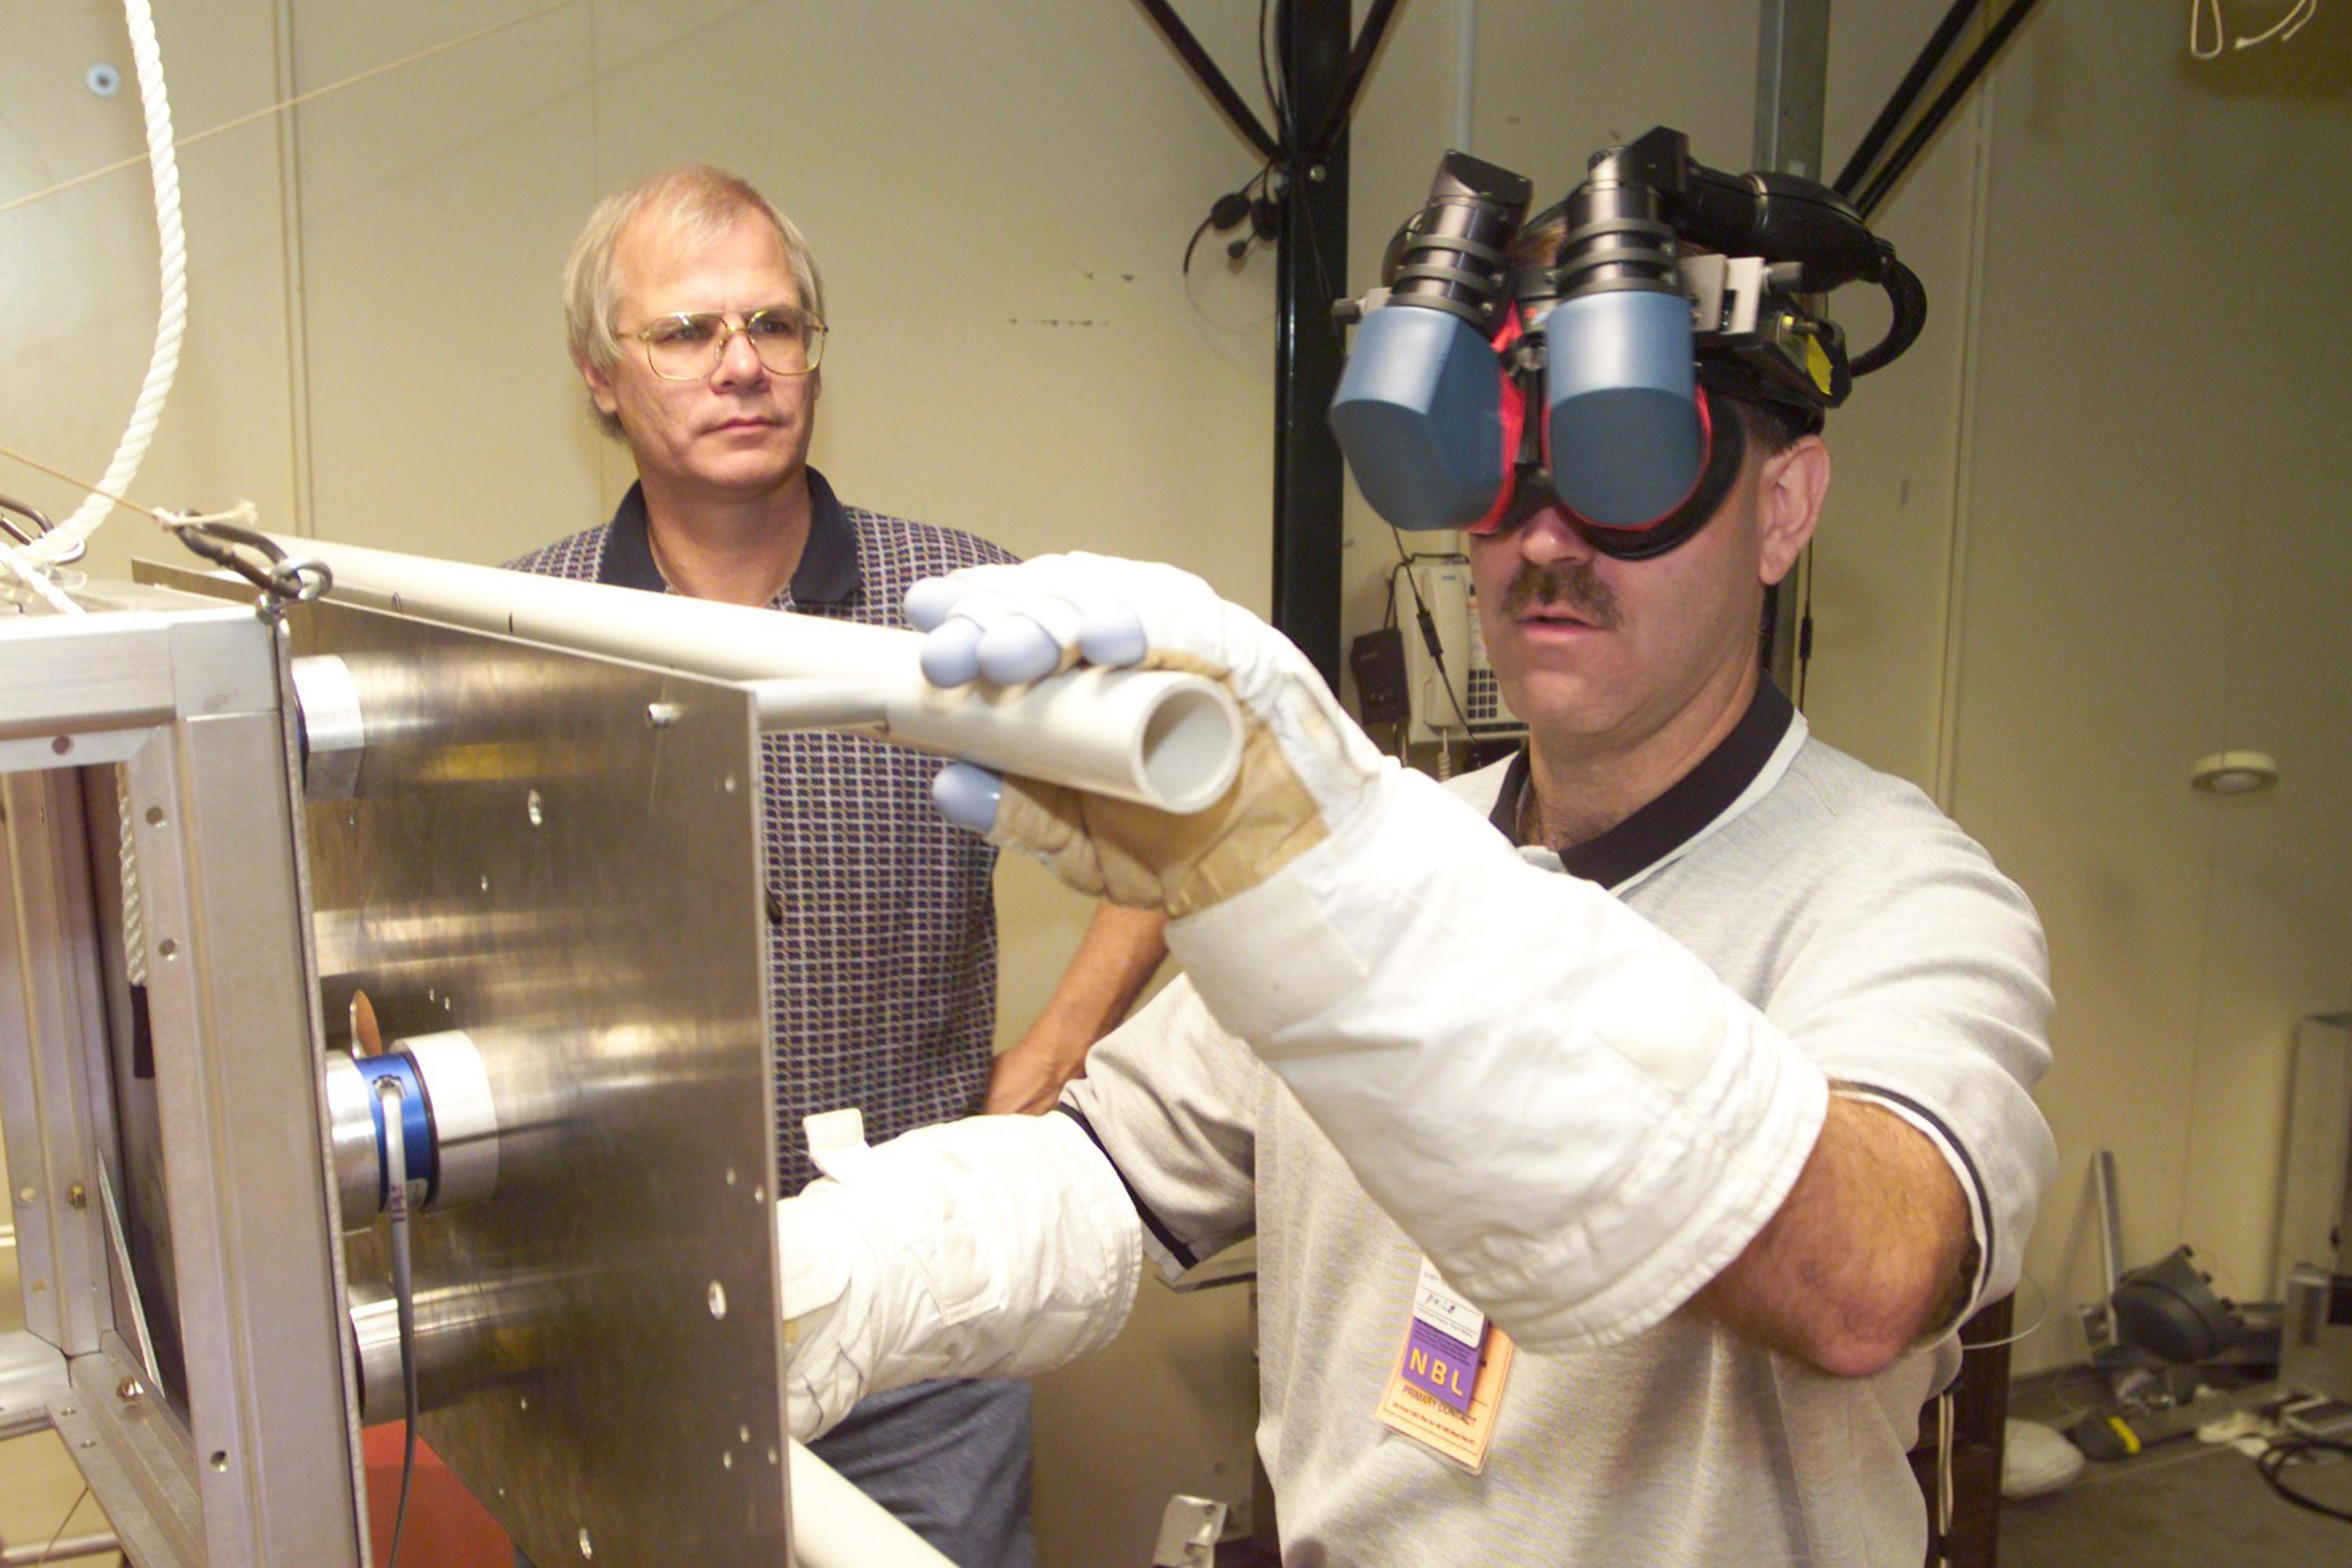
\includegraphics[width=0.45\textwidth]{figures/future-mill.jpg}
  \caption{Grad student tests new virtual reality mill}
  \label{fig:vr-mill}
\end{figure}

\subsection{Subvert Academic Thought}
\todo{Pivot academic thought away from mathematical and computational problems.
Wasted  brainpower when they could be thinking about products and brands.}

\subsection{ACM Seizes Means of Production}
\todo{By putting crushed crystals in CEO's coffee, the ACM will influence CEOs
  to liquidate their companies and give them to the ACM.
  The mills were originally for crushing crystals but after the revolution they
were re purposed to generate electricity
ESPN executives are Mormon though and impervious to crystal healing and coffee. So we had to compromise: the entire National Park System became an ESPN Zone.
}

\subsection{Future Work}
A consequence of the invention of time travel \cite{time-travel} and the vanity
of engineers (not scientests) \todo{Cite ubiquity article} is that people
keep going further back in time to give themselves credit for the invention of
the time machine.
However, we propose to go back in time for a different reason.
To put a stop to the Open Adcess.
To put a stop to the work dungeons.
And to put a stop to the ACM Revolution, which however noble in it's initial
goals has become  kinda lame.
We will open a mill based on anarchist principles that welcomes all to come and
mill and share healing crystals.
Our report of our screwing missadventuresduring our fieldtrip into the past can
be seen in the latest edition of \textit{Ubiquity} \cite{future-ub}.

\todo{Servers powered by manual labor (guy in basement pushing bar around).  If
you want an ad free version you can visit your local ACM work dungeon to
manually turn a generator.)}


\todo{Set system clock to run 10 to the 8 times slower than real time for
reporting performance numbers as recommended by
https://queue.acm.org/detail.cfm?id=3036398}


\section{Conclusion}


\end{document}
